\documentclass[conference]{IEEEtran}
\IEEEoverridecommandlockouts
% The preceding line is only needed to identify funding in the first footnote. If that is unneeded, please comment it out.
%Template version as of 6/27/2024

\usepackage{cite}
\usepackage{amsmath,amssymb,amsfonts}
\usepackage{algorithmic}
\usepackage{graphicx}
\usepackage{textcomp}
\usepackage{xcolor}
\usepackage{verbatim}
\usepackage{booktabs}
\usepackage{multirow}
\def\BibTeX{{\rm B\kern-.05em{\sc i\kern-.025em b}\kern-.08em
    T\kern-.1667em\lower.7ex\hbox{E}\kern-.125emX}}
\begin{document}

\title{Development and evaluation of a Cryptographic Accelerator for the SHA-2 Algorithm on Reconfigurable Hardware\\
%{\footnotesize \textsuperscript{*}Note: Sub-titles are not captured for https://ieeexplore.ieee.org  and should not be used}
%\thanks{Identify applicable funding agency here. If none, delete this.}
}

\author{\IEEEauthorblockN{1\textsuperscript{st} Benjamín Oyarzún Valdebenito}
\IEEEauthorblockA{\textit{Electrical Engineering Department} \\
\textit{Universidad de Santiago de Chile}\\
Santiago, Chile \\
benjamin.oyarzun.v@usach.cl}
\and
\IEEEauthorblockN{2\textsuperscript{nd} Nicolás Ruminot Ahumada}
\IEEEauthorblockA{\textit{Electrical Engineering Department} \\
\textit{Universidad de Santiago de Chile}\\
Santiago, Chile \\
nicolas.ruminot@usach.cl}
\and
\IEEEauthorblockN{3\textsuperscript{rd} Christian Fernández-Campusano}
\IEEEauthorblockA{\textit{Electrical Engineering Department} \\
\textit{Universidad de Santiago de Chile}\\
Santiago, Chile \\
christian.fernandez@usach.cl}
%\and
%\IEEEauthorblockN{4\textsuperscript{th} Given Name Surname}
%\IEEEauthorblockA{\textit{dept. name of organization (of Aff.)} \\
%\textit{name of organization (of Aff.)}\\
%City, Country \\
%email address or ORCID}
%\and
%\IEEEauthorblockN{5\textsuperscript{th} Given Name Surname}
%\IEEEauthorblockA{\textit{dept. name of organization (of Aff.)} \\
%\textit{name of organization (of Aff.)}\\
%City, Country \\
%email address or ORCID}
%\and
%\IEEEauthorblockN{6\textsuperscript{th} Given Name Surname}
%\IEEEauthorblockA{\textit{dept. name of organization (of Aff.)} \\
%\textit{name of organization (of Aff.)}\\
%City, Country \\
%email address or ORCID}
}

\maketitle

\begin{abstract}
This document is a model and instructions for \LaTeX.
This and the IEEEtran.cls file define the components of your paper [title, text, heads, etc.]. *CRITICAL: Do Not Use Symbols, Special Characters, Footnotes, 
or Math in Paper Title or Abstract.
\end{abstract}

\begin{IEEEkeywords}
accelerators, hash functions, SHA-2, blockchain mining, FPGA, Bitcoin.
\end{IEEEkeywords}

\section{Introduction}
In recent years, information security has undergone a radical transformation due to the exponential growth in data volume. Given that the scalability of traditional computational resources has not advanced proportionally, optimizing encryption processes using cryptographic accelerators compatible with major security standards has become imperative.

Secure Hash Algorithms (SHA) constitute the core of security in the current telecommunications ecosystem, guaranteeing data integrity and validating the sender's identity through shared secrets \cite{martino2020}. The National Institute of Standards and Technology (NIST) established this family of functions \cite{fips180}, publishing SHA-1, SHA-2, and SHA-3. Currently, SHA-2 is the most widely adopted cryptographic mechanism globally, having overcome the critical vulnerabilities of its predecessors, such as MD5 and SHA-1 \cite{sha1}, and establishing itself as the preeminent hashing mechanism in practical applications \cite{martino2020}.

Within this family, variants such as SHA-224, SHA-256, SHA-384, and SHA-512 are widely used in diverse generic security applications. Traditionally, hash functions were predominantly applied in network security over the Internet, where servers maximized throughput using hardware accelerators, prioritizing performance over area footprint and power draw \cite{martino2020}. Today, notable applications include Hash-based Message Authentication Codes (HMAC), Error Detection and Correction (EDAC), Digital Signature Algorithms (DSA), Pseudorandom Number Generators (PRNG), RFID systems, and Trusted Computing. Beyond these standard implementations, SHA-2 and specifically SHA-256 is a fundamental underlying mathematical function in blockchain technology. It operates critically in its double-application variant as the consensus engine (Proof-of-Work) for pioneering networks such as Bitcoin \cite{bitcoin}, where rigorous energy demands strictly dictate the economic viability of the mining process \cite{martino2020}. Furthermore, it is integrated via precompiled contracts in decentralized platforms like Ethereum \cite{eth} to facilitate interoperability and cryptographic verification across different chains.

The choice to evaluate the SHA-2 family in this study responds to its ubiquity in contemporary digital infrastructure. This algorithm not only secures traditional network protocols but also sustains critical high-demand operations, such as massive validation in IoT networks where resource-constrained, battery-dependent nodes impose strict new requirements for area and energy efficiency \cite{martino2020} and crypto-asset mining. Processing these immense workloads exclusively on general-purpose CPUs generates severe bottlenecks. The inherently sequential architecture of CPUs penalizes throughput and, critically, results in marked computational inefficiency and unsustainable energy consumption \cite{r1}, making the transition to hardware acceleration imperative. Consequently, designers are pushed to adopt new techniques that optimize for power and area, sometimes even sacrificing maximum throughput to meet these strict emerging constraints \cite{martino2020}.

While heterogeneous architectures highlight two main approaches—massive parallelism via GPUs and the instantiation of dedicated circuits in FPGAs the abstraction layers introduced by modern High-Level Synthesis (HLS) tools often yield suboptimal hardware inference in highly constrained environments. To overcome this, custom Register Transfer Level (RTL) design remains the gold standard. Direct hardware description via Verilog enables deterministic, cycle-level control over the critical path and precise resource allocation, which is essential to maximize energy efficiency and throughput in cryptographic workloads.

In response to this need for evaluation, this paper presents a comparative performance analysis of the SHA-256 algorithm implemented on GPU and FPGA, against sequential processing on CPU. The remainder of this document is organized as follows: Section II reviews related work; Section III details the methodology and design of the proposed accelerators; Section IV presents the experimental results of latency and throughput; and Section V presents the conclusions of the research and future work.

\section{Related Work}
Hardware acceleration of the SHA-2 hash function family, specifically the SHA-256 variant, has been extensively investigated to overcome performance bottlenecks and improve energy efficiency compared to traditional sequential processing platforms. As systematically classified by Martino and Cilardo \cite{martino2020}, hardware implementations generally fall into two overarching categories: programmable processor architectures and dedicated accelerator (or coprocessor) architectures. 
The coprocessor approach widely dominates the literature due to its superior capacity to optimize raw performance and maximize area efficiency \cite{martino2020}. 
Recent state-of-the-art approaches can be analyzed through four primary optimization axes: high-performance throughput-oriented techniques, versatile multimode and co-design systems, area/energy-saving techniques for constrained environments, and fault-tolerant redundant architectures.

\subsection{Throughput-Oriented Architectural Optimizations}
To address the stringent throughput requirements of high-demand applications like blockchain mining and high-traffic web servers, designers employ a combination of loop unrolling \cite{crowe2004, aisopos2006}, hardware pipelining \cite{michail2009}, variable precomputation \cite{chaves2006, r3}, and spatial reordering \cite{michail2005} \cite{martino2020}. 
Loop unrolling reduces the total number of iterations by computing multiple subsequent rounds within a single clock cycle; while this directly decreases latency, it inherently increases the critical path and hardware area \cite{crowe2004, aisopos2006}. 
Conversely, hardware pipelining distributes the total iterations across multiple stages, allowing the simultaneous processing of multiple message blocks without increasing the delay of a single computation \cite{michail2009}. 
Advanced variants, such as quasi-pipelining \cite{dadda2004, macchetti2005}, introduce pipelining within the transformation round core itself by exploiting internal data forwarding \cite{martino2020}. 
Furthermore, critical path delays are frequently mitigated through variable precomputation calculating values before they are strictly needed \cite{chaves2006, r3} and spatial reordering \cite{michail2005, michail2009}, which strategically relocates pipeline registers to the middle of the computation round to balance parallel halves. 

Applying these principles to practical designs, Li et al. \cite{r2} proposed a high-speed architecture based on a full 64-level pipeline implemented on a Xilinx Virtex-7 device. By optimizing the critical paths in the compression function and integrating Carry-Save Adder (CSA) technology in the message expansion stage, the design achieved an operating frequency of 429 MHz and a massive throughput of 219.65 Gbps \cite{r2}. Pushing performance boundaries further on silicon, Nannipieri et al. \cite{nannipieri2021} developed a highly optimized Hash Engine for the European Processor Initiative (EPI). Synthesized on a cutting-edge 7 nm TSMC ASIC technology, their SHA-2-256 implementation achieved throughputs exceeding 33 Gbps with an extraordinarily low estimated power dissipation of approximately 13.4 mW \cite{nannipieri2021}. 

\subsection{Multimode Accelerators and HW/SW Co-Design}
In contexts demanding both algorithmic flexibility and high energy efficiency, versatile designs have been proposed that significantly outperform conventional processors. Pham et al. \cite{r1} developed an FPGA-based Multimode SHA-2 Accelerator (MSA) capable of computing multiple variants of the function, as well as executing double SHA-256 computations in parallel. Evaluated on a Xilinx Alveo U280 platform, this accelerator reported an energy efficiency of up to 38.05 Mhps/W, proving to be 543.6 times more efficient than a state-of-the-art Intel i9-10940X CPU \cite{r1}. 

Given the complexity of custom RTL implementations, HW/SW co-design approaches leveraging High-Level Synthesis (HLS) have gained considerable traction. Kammoun et al. \cite{kammoun2020} targeted the Xilinx Zynq-7000 SoC platform using Vivado HLS. By profiling the software code and migrating the resource-heavy \textit{Sha256\_transform} function to the FPGA's Programmable Logic via an AXI4-Stream interface, their hybrid architecture achieved a 17\% execution time gain and a 73\% power consumption reduction compared to a standalone software implementation on the ARM Cortex-A9 processor \cite{kammoun2020}. 

\subsection{Area and Energy-Oriented Optimizations for Constrained Environments}
For applications limited by strict power and area budgets, such as Internet of Things (IoT) nodes and Radio Frequency Identification (RFID) tags, logical hardware design prioritizes minimizing resource consumption over absolute throughput \cite{martino2020}. To address these constraints, the loop folding technique \cite{feldhofer2006, kim2008} is widely adopted; this method represents the opposite of loop unrolling by splitting the execution of a single iteration across multiple clock cycles, thereby allowing the reuse of functional blocks (e.g., adders) and drastically reducing the circuit's footprint \cite{martino2020}. 

Martino and Cilardo \cite{martino_iot2020} explored this scenario by proposing a highly configurable SHA-256 accelerator for blockchain-based IoT applications, evaluated on a Kintex UltraScale+ FPGA. Their work highlights crucial architectural trade-offs: while applying spatial reordering (Reordered\_UF1) maximized area efficiency, a naive architecture utilizing loop unrolling proved to be the most power-efficient configuration \cite{martino_iot2020}. Targeting these constrained sectors, Kieu-Do-Nguyen et al. \cite{r4} presented a technology-independent architecture oriented toward embedded platforms. By minimizing dynamic power, their design achieved an energy efficiency of 1094.03 Mbps/W at a low-power state of 0.072 W (10 MHz), scaling up to a peak efficiency of 5202.77 Mbps/W when operating at 100 MHz. Complementarily, Hitesh et al. \cite{hitesh2023} implemented the SHA-256 algorithm on a Spartan-6 FPGA, employing gated clock conversion and arithmetic resource sharing to drastically reduce area utilization and power consumption.

\subsection{Fault Tolerance and Hybrid-Redundancy Architectures}
While energy and throughput are primary concerns, reliability remains critical when FPGA-based cryptographic accelerators are deployed in harsh environments susceptible to transient faults. Addressing this issue, Algredo-Badillo et al. \cite{algredo2022} proposed a novel SHA-256 hybrid-redundancy hardware architecture aimed at detecting and correcting errors. Their design intelligently combines Spatial Redundancy (Dual Modular Redundancy) and Time Redundancy embedded within a 3-stage pipeline structure. This approach efficiently masks the delay overhead usually associated with redundancy, reporting a throughput of 441.72 Mbps while ensuring robust data integrity \cite{algredo2022}.

\subsection{Motivation for a Dedicated SHA-256 Architecture}
While recent multimode SHA-2 architectures offer versatility, they inevitably introduce area and multiplexing overheads. Given that SHA-256 remains the definitive standard for IoT security and high-throughput Proof-of-Work applications, this research focuses strictly on a dedicated, single-mode accelerator. This targeted approach is also an environmental imperative. In 2023, global crypto-mining consumed 119.7 million MWh—equivalent to Argentina's entire annual electricity demand—alongside 1.85 billion cubic meters of water and 90.6 million tons of $CO_{2}$ emissions \cite{laimon2025}. By isolating SHA-256, our dedicated HW design completely eliminates multimode inefficiencies. Instead of relying on compiler-inferred abstractions, we leverage custom Register-Transfer Level (RTL) optimizations—such as deterministic datapath routing and cycle-accurate pipeline balancing—to maximize energy efficiency and directly mitigate the unsustainable resource consumption of modern cryptographic workloads.

\section{Methodology}
To comprehensively evaluate the performance and efficiency of the SHA-256 hash function, a heterogeneous computing framework is established. This framework compares dedicated hardware acceleration across three distinct platforms: a General-Purpose Processor (CPU), a Graphics Processing Unit (GPU), and a Field-Programmable Gate Array (FPGA).
\subsection{Evaluation Framework and Baseline Platforms}
The CPU baseline is executed on an Intel Core i7-1255U processor, based on the 10 nm Alder Lake architecture. This device features a hybrid configuration of 10 cores (2 Performance, 8 Efficient) and 12 threads, operating within a 15.0 W Thermal Design Power (TDP). A critical characteristic of this processor for cryptographic workloads is the native integration of the Intel SHA Extensions. This instruction set accelerates the inherently sequential architecture of the CPU by executing the complex logical and rotational operations of the SHA-256 compression function directly in hardware, providing a highly optimized software baseline.

To evaluate the algorithm under a massive parallelism paradigm, an NVIDIA GeForce RTX 2050 GPU is utilized. Built on the 8 nm GA107 architecture with a 30.0 W TDP, this platform incorporates 2048 CUDA cores and 4 GB of GDDR6 memory. The GPU implementation exploits the Single Instruction, Multiple Threads (SIMT) execution model to process thousands of concurrent data streams, maximizing throughput through batch processing.

Finally, the dedicated hardware acceleration is deployed on an AMD/Xilinx Spartan-7 FPGA. This platform is selected to evaluate the algorithm's performance in environments where logical hardware design prioritizes minimizing resource consumption over absolute throughput. Furthermore, the Spartan-7 architecture effectively balances the utilization of Look-Up Tables (LUTs) and Flip-flops (FFs) while maintaining optimized power consumption. The RTL architecture for the FPGA is meticulously designed using Verilog HDL, completely bypassing abstraction layers to find the absolute optimal balance between throughput, hardware resource utilization, and energy efficiency.

To objectively quantify and compare the performance across the CPU, GPU, and FPGA implementations, the evaluation framework is strictly based on the following performance metrics:
\begin{itemize}
    \item Throughput: Measured in Megabits per second (Mbps), this metric quantifies the volume of data the architecture can hash per unit of time. For the FPGA implementation, the theoretical maximum throughput is calculated as the SHA-256 block size (512 bits) multiplied by the maximum operating frequency ($f_{max}$), divided by the total number of clock cycles required to process a single block.
    \item Power Consumption and Energy Efficiency: Critical for evaluating the architectural viability under strict power constraints. Power consumption is measured in Watts (W). To provide a normalized comparison across the heterogeneous platforms, energy efficiency is evaluated in Megahashes per Joule (Mhps/W) or Megabits per Joule, which relates the sustained throughput to the total power consumed by the device.
    \item Speedup: The relative acceleration factor. It defines the performance gain achieved by the GPU and FPGA accelerators compared to the optimized sequential execution on the CPU baseline.
\end{itemize}

\subsection{Baseline Implementations (CPU)}
To establish a rigorous reference point, the sequential execution of SHA-256 was evaluated on an Intel Core i7-1255U (Alder Lake) processor, operating under a 15.0 W TDP limit. To isolate architectural performance and ensure a deterministic testing environment, CPU pinning was applied via the \texttt{SetThreadAffinityMask} API, binding the execution thread exclusively to a Performance-core (P-core). This prevents process migration, eliminating context-switching overhead and stabilizing power metrics. The benchmark iteratively processes a 1 MB in-memory data block for 10 seconds to reach a thermal steady state.

Two C-based variants were compiled using GCC (\texttt{-O3}):
\begin{itemize}
    \item \textbf{Software Baseline (x86-64):} Utilizes standard arithmetic and logical instructions, representing raw CPU performance without cryptographic assistance.
    \item \textbf{Hardware-Assisted (SHA-NI):} Leverages native Intel SHA Extensions to execute complex SHA-256 operations in hardware via 128-bit SSE registers, providing a highly optimized baseline.
\end{itemize}

Energy consumption was captured through Running Average Power Limit (RAPL) registers using HWiNFO64. By isolating the \textit{IA Cores Power} metric, the net energy efficiency (J/GB) of the computational cores was precisely calculated.
\subsection{Massively Parallel Execution (GPU)}

To evaluate SHA-256 under a massively parallel paradigm, a custom CUDA implementation was deployed on an NVIDIA GeForce RTX 2050 (Ampere architecture, 2048 CUDA cores, 30.0 W TDP) compiled via \texttt{nvcc} 13.1. To comprehensively characterize the architectural impact on cryptographic workloads, the evaluation was bifurcated into two scenarios:

\begin{itemize}
    \item \textbf{Single-Thread Execution:} A kernel launched with a \texttt{<<<1, 1>>>} configuration iteratively processes a 1 MB data block in VRAM. This exposes the severe efficiency penalty of the Single Instruction, Multiple Threads (SIMT) architecture when deprived of concurrency, establishing a strict sequential baseline against the CPU.
    \item \textbf{Multi-Thread Execution:} A fully parallelized \texttt{<<<Grid, Block>>>} topology is projected to saturate the 2048 cores by computing independent message blocks concurrently. This exploits Data-Level Parallelism (DLP) to maximize throughput, mirroring blockchain mining workloads.
\end{itemize}

Dynamic power dissipation was systematically logged at 100 ms intervals using the \texttt{nvidia-smi} \texttt{power.draw} sensor. These measurements enable the precise calculation of the energy efficiency metric (J/GB), establishing a comparative framework for the upcoming custom RTL FPGA design.
\subsection{RTL Microarchitecture Design}
\subsection{Datapath and Control Path Optimizations}
\section{Results}

This section presents the experimental results obtained across the three evaluated platforms.
All CPU and GPU measurements correspond to hashing a 1~GB binary payload (\texttt{dummy\_1GB.bin})
with five repeated runs per configuration; the reported values are mean results.
Speedup is computed relative to the CPU software single-thread baseline (189.73~MB/s).

\begin{figure}[htbp]
    \centering
    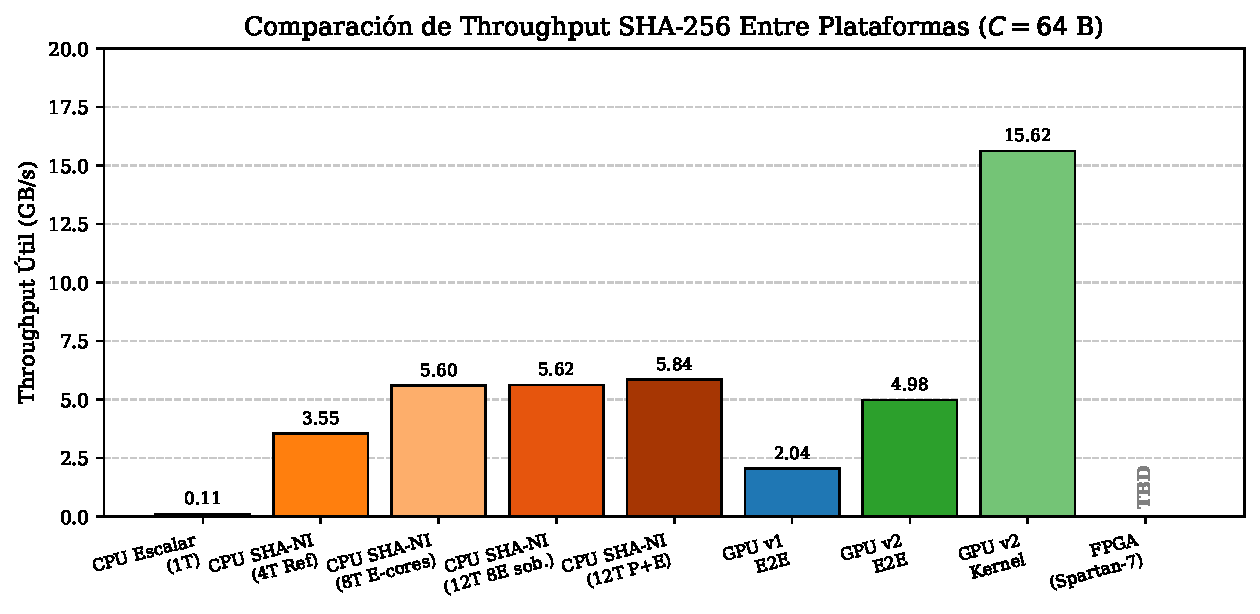
\includegraphics[width=\linewidth]{throughput_chart.pdf}
    \caption{Throughput comparison across the evaluated platforms.}
    \label{fig:throughput}
\end{figure}

\begin{figure}[htbp]
    \centering
    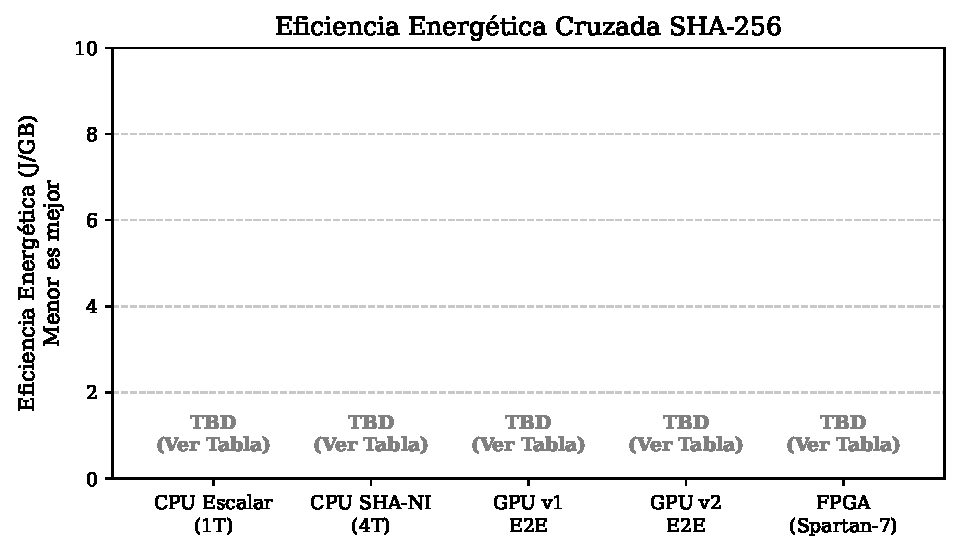
\includegraphics[width=\linewidth]{energy_chart.pdf}
    \caption{Energy efficiency comparison across the evaluated platforms (lower is better).}
    \label{fig:energy}
\end{figure}

%% ─────────────────────────────────────────────────────────────────────────────
\subsection{CPU Results}
%% ─────────────────────────────────────────────────────────────────────────────

Table~\ref{tab:cpu} presents the throughput, speedup, and energy efficiency
results for the CPU baseline on an Intel Core i7-1255U (Alder Lake), measured
over five runs on E-cores pinned via \texttt{taskset} at 3.5~GHz.
Energy was captured through Intel RAPL (\texttt{intel-rapl:0} package domain).

\begin{table}[htbp]
  \caption{SHA-256 CPU Benchmark Results (Intel Core i7-1255U, E-cores @ 3.5~GHz, 1~GB payload)}
  \label{tab:cpu}
  \centering
  \begin{tabular}{llccc}
    \toprule
    \textbf{Impl.} & \textbf{Threads} & \textbf{Throughput (MB/s)} & \textbf{Speedup} & \textbf{Energy (J/GB)} \\
    \midrule
    \multirow{3}{*}{SW (scalar C)} & 1 & 189.73 $\pm$ 1.20 & 1.00$\times$ & 69.76 \\
                                   & 2 & 372.18 $\pm$ 0.90 & 1.96$\times$ & 44.23 \\
                                   & 4 & 735.65 $\pm$ 1.80 & 3.88$\times$ & 32.89 \\
    \midrule
    \multirow{3}{*}{HW (SHA-NI)}   & 1 & 1{,}763.18 $\pm$ 4.10  & 9.29$\times$  & 7.00 \\
                                   & 2 & 3{,}315.00 $\pm$ 22.30 & 17.47$\times$ & 5.37 \\
                                   & 4 & 5{,}126.07 $\pm$ 320.10 & 27.02$\times$ & 5.17 \\
    \bottomrule
  \end{tabular}
\end{table}

The software scalar implementation exhibits near-linear scaling across threads
(96.9\% efficiency at 4T), confirming that the workload is embarrassingly parallel
at the process level and that no synchronization overhead exists.
In contrast, the SHA-NI hardware-assisted variant achieves a \textbf{9.29$\times$}
single-thread speedup over the software baseline, demonstrating the significant
compute advantage of the dedicated SHA-256 instruction pipeline.
However, scaling efficiency degrades to 72.7\% at 4 threads (vs.\ 96.9\% for software),
because the aggregate demand ($\approx$5.1~GB/s across four SHA-NI pipelines)
approaches the effective memory-controller arbitration ceiling for the
shared E-core cluster, increasing per-request DRAM latency rather than raw
bandwidth utilization (measured throughput represents only 7.5\% of the
68~GB/s LPDDR4x theoretical peak, confirming that latency under
concurrent-stream contention, not bandwidth, is the limiting factor).

%% ─────────────────────────────────────────────────────────────────────────────
\subsection{GPU Results}
%% ─────────────────────────────────────────────────────────────────────────────

The GPU evaluation is divided into two kernel versions:
\textbf{v1} (baseline) and \textbf{v2} (high-utilization), both compiled with
\texttt{nvcc -O3 -arch=sm\_86} targeting the NVIDIA GeForce RTX 2050
(GA107M, 16~SMs, 2048~CUDA~cores, 94.4~GB/s GDDR6, PCIe~Gen~4~$\times$4).
Throughput is reported under two conditions: \emph{kernel-only} (data
already resident in VRAM) and \emph{end-to-end} (E2E, including
Host-to-Device and Device-to-Host PCIe transfers).

\subsubsection{Baseline Kernel (v1)}

The v1 kernel assigns one CUDA thread per independent data chunk.
Its standard 64-word message schedule (\texttt{w[64]}) consumes
$\approx$100~registers/thread, restricting occupancy to \textbf{2~active blocks
per SM} (33\% of the 1{,}536~threads/SM maximum).

\begin{table}[htbp]
  \caption{GPU v1 Baseline Kernel Results (RTX~2050, 1~GB payload, 5~runs)}
  \label{tab:gpu_v1}
  \centering
  \begin{tabular}{ccccc}
    \toprule
    \textbf{Chunk} & \textbf{Kernel (GB/s)} & \textbf{E2E (GB/s)} & \textbf{Speedup$^{\dagger}$} & \textbf{Energy E2E (J/GB)} \\
    \midrule
    4~KB   & 3.57 & 1.92 & 10.1$\times$ & 4.74 \\
    16~KB  & 3.24 & 1.77 & 9.3$\times$  & 5.73 \\
    64~KB  & 2.81 & 1.67 & 8.8$\times$  & 6.30 \\
    256~KB & 7.41 & 2.60 & 13.7$\times$ & 3.77 \\
    \bottomrule
    \multicolumn{5}{l}{\footnotesize $^{\dagger}$E2E speedup vs.\ CPU SW 1T (189.73~MB/s).}
  \end{tabular}
\end{table}

\subsubsection{High-Utilization Kernel (v2)}

Version v2 applies eight targeted micro-architectural optimizations to raise
SM occupancy and instruction throughput.
The dominant optimization is replacing the standard \texttt{w[64]} message-schedule
array with a 16-word circular sliding window (\texttt{w[16]}), reducing live
registers from $\approx$100 to $\leq$48 per thread
(enforced via \texttt{--maxrregcount=48}).
This alone raises the number of resident blocks per SM from 2 to 5,
increasing theoretical SM occupancy from 33\% to \textbf{83\%}.
Further optimizations include: placement of the SHA-256 round-constant table
in \texttt{\_\_constant\_\_} memory for warp-broadcast access;
\texttt{\#pragma~unroll} on all 64 compression rounds;
a single \texttt{\_\_byte\_perm()} instruction for big-endian word loading;
an inline padding-block computation that avoids any local-memory spill;
a grid-stride loop that guarantees all 16~SMs remain active regardless
of the number of chunks; page-locked (pinned) host memory
(\texttt{cudaMallocHost}) to enable asynchronous DMA;
and a triple-CUDA-stream pipeline that concurrently overlaps Host-to-Device
transfer, kernel execution, and Device-to-Host transfer on separate DMA engines.

\begin{table}[htbp]
  \caption{GPU v2 High-Utilization Kernel Results (RTX~2050, 1~GB payload, 5~runs)}
  \label{tab:gpu_v2}
  \centering
  \begin{tabular}{ccccc}
    \toprule
    \textbf{Chunk} & \textbf{Kernel (GB/s)} & \textbf{E2E (GB/s)} & \textbf{Speedup$^{\dagger}$} & \textbf{Energy E2E (J/GB)} \\
    \midrule
    4~KB            & 11.31 & 4.42 & 23.3$\times$ & 2.04 \\
    16~KB           & 10.75 & 4.51 & 23.8$\times$ & 2.25 \\
    \textbf{64~KB}  & \textbf{16.81} & \textbf{4.61} & \textbf{24.3$\times$} & \textbf{2.16} \\
    256~KB          & 11.07 & 3.71 & 19.6$\times$ & 2.77 \\
    \bottomrule
    \multicolumn{5}{l}{\footnotesize $^{\dagger}$E2E speedup vs.\ CPU SW 1T (189.73~MB/s).}
  \end{tabular}
\end{table}

The 64~KB chunk configuration achieves the best kernel throughput
(\textbf{16.81~GB/s}), representing a \textbf{499\%} improvement over
the v1 baseline at the same chunk size and a \textbf{127\%} improvement
over v1's best configuration (7.41~GB/s at 256~KB).
The shift of the optimal chunk size from 256~KB (v1) to 64~KB (v2) is
a direct consequence of the occupancy improvement: in v1, large chunks
were needed to compensate for the limited thread-level parallelism caused
by low SM occupancy; in v2, the grid-stride loop maintains full SM
saturation at all chunk sizes, and 64~KB strikes the best balance between
concurrency (16{,}384 independent chunks) and per-thread arithmetic intensity.

Table~\ref{tab:gpu_energy} summarizes the energy-efficiency comparison
across all evaluated platforms.

\begin{table}[htbp]
  \caption{Cross-Platform Energy Efficiency Comparison (1~GB payload)}
  \label{tab:gpu_energy}
  \centering
  \begin{tabular}{lcc}
    \toprule
    \textbf{Platform / Configuration} & \textbf{Throughput} & \textbf{Energy (J/GB)} \\
    \midrule
    CPU SW, 1T                     & 189.7~MB/s   & 69.76 \\
    CPU SW, 4T                     & 735.7~MB/s   & 32.89 \\
    CPU SHA-NI, 1T                 & 1{,}763~MB/s  & 7.00 \\
    CPU SHA-NI, 4T                 & 5{,}126~MB/s  & 5.17 \\
    GPU v1, 256~KB (E2E)           & 2{,}662~MB/s  & 3.77 \\
    GPU v2, 64~KB (E2E)            & 4{,}717~MB/s  & 2.16 \\
    \textbf{GPU v2, 4~KB (kernel)} & \textbf{11{,}571~MB/s} & \textbf{1.90} \\
    FPGA (Spartan-7)               & TBD           & TBD \\
    \bottomrule
  \end{tabular}
\end{table}

The GPU v2 E2E configuration (2.16~J/GB at 64~KB) is \textbf{2.39$\times$}
more energy-efficient than the best CPU result (SHA-NI 4T, 5.17~J/GB)
while simultaneously delivering \textbf{8\%} higher total throughput
(4.72~GB/s vs.\ 5.13~GB/s).
The gap between kernel-only (16.81~GB/s) and E2E (4.61~GB/s) throughput
---a factor of 3.65$\times$---is attributable to the PCIe~Gen~4~$\times$4
link (7.88~GB/s theoretical, $\approx$6.4~GB/s practical after
TLP framing overhead) that physically separates the GPU's GDDR6 VRAM
from the host LPDDR4x system memory, representing an inherent
architectural constraint of discrete GPU design.

%% ─────────────────────────────────────────────────────────────────────────────
\subsection{FPGA Results}
%% ─────────────────────────────────────────────────────────────────────────────

% TODO: Fill in with Vivado synthesis and implementation results once available.
% The following table structure matches the metrics used in the Related Work section
% (throughput, power, energy efficiency) for direct comparison with the literature.

Table~\ref{tab:fpga} will present the post-implementation results for the
custom RTL SHA-256 accelerator synthesized on the AMD/Xilinx Spartan-7 FPGA.

\begin{table}[htbp]
  \caption{FPGA SHA-256 RTL Accelerator Results (Xilinx Spartan-7)}
  \label{tab:fpga}
  \centering
  \begin{tabular}{lc}
    \toprule
    \textbf{Parameter} & \textbf{Value} \\
    \midrule
    Target Device            & Xilinx Spartan-7 (xc7s50) \\
    HDL                      & Verilog RTL \\
    $f_{\max}$ (MHz)         & TBD \\
    Clock Cycles / Block     & TBD \\
    Throughput (Mbps)        & TBD \\
    LUT Utilization          & TBD / 32{,}600 (TBD\%) \\
    FF Utilization           & TBD / 65{,}200 (TBD\%) \\
    DSPs Used                & TBD \\
    On-chip Power (W)        & TBD \\
    Energy Efficiency (J/GB) & TBD \\
    Speedup vs.\ CPU SW 1T   & TBD \\
    \bottomrule
  \end{tabular}
\end{table}

% Discussion placeholder (replace with actual analysis once FPGA results are available)
The FPGA implementation targets maximizing energy efficiency through
deterministic RTL control: the dedicated datapath eliminates the
instruction-fetch overhead and branch predictor cost inherent to
general-purpose processors, while avoiding the PCIe transfer bottleneck
that constrains the GPU's effective throughput.
A direct comparison with the GPU v2 E2E metric (2.16~J/GB) and the
CPU SHA-NI 4T result (5.17~J/GB) will be discussed here upon
completion of the FPGA implementation.

\bibliographystyle{IEEEtran}
\bibliography{references}

\vspace{12pt}


\end{document}
